\documentclass[10pt]{paper}
\usepackage[a4paper, total={6in, 9in}, bottom = 1in]{geometry}
\usepackage[utf8]{inputenc}
\usepackage[slovak]{babel}
\usepackage{fancyhdr}
\usepackage{mathtools}
\usepackage{pgfplots}
\usepackage{wrapfig}
\usepackage{amsmath}
\usepackage{algpseudocode}
\usepackage{paracol}
\newcommand{\name}{Katarína Kejstová 433820, Viktória Vozárová 433334}
\newcommand{\datum}{Projekt IV109}
\pagestyle{fancy}
\fancyhf{}
\lhead{\name}
\rhead{\datum}
\setlength\parindent{0pt}
\begin{document}

\begin{titlepage}
\begin{center}
  \bfseries
  \huge Záverečná správa
  \vskip.2in
  \textsc{\LARGE projektu IV109 }
  \vskip1in
  \emph{\huge Robot - zbieranie pokladu}
\end{center}

\vskip3in

\begin{minipage}{.45\textwidth}
  \begin{flushleft}
    \bfseries\large Prednášajúci:\par \emph{doc. Mgr. Radek Pelánek, Ph.D.}
  \end{flushleft}
\end{minipage}
\hskip.15\textwidth
\begin{minipage}{.40\textwidth}
  \begin{flushleft}
    \bfseries\large Študenti:\par \emph{Katarína Kejstová} 433820 \par \emph{Viktória Vozárová} 433334
  \end{flushleft}
\end{minipage}

\vskip1.3in

\centering
\bfseries
\Large Jarný semester 2016
\end{titlepage}

\section{Zadanie projektu}

\textit{Variace na příklad zmíněný na přednášce. Robot se pohybuje v čtvercové mřížce, na některých polích jsou poklady, které má posbírat, případně zdi, díry, a pod. Vytvořte genetický algoritmus, který bude vytvářet navigační kód pro robota (tak aby posbíral co nejvíce pokladu).}

\section{Genetické algoritmy}
 
Genetické algoritmy sú vo všeobecnosti heuristické postupy, aplikujúce princípy z evolučnej biológie. Často sú využívané na riešenia zložitých problémov, pretože sú schopné vytvoriť netriviálne (náhodné) riešenia. Než začneme s popisom nášho riešenia problému, je potrebné definovať niektoré pojmy spájajúce sa s genetickými algoritmami a ich aplikáciou v praxi.\\

\textbf{Chromozóm}

V aplikácii genetických algoritmov je chromozóm chápaný ako reťazec, resp. postupnosť symbolov, reprezentujúci jedinca s výslednými vlastnosťami. Každá vlastnosť nejako popisuje riešenie a preto reťazec chápeme ako riešenie.\\

\textbf{Gén}

Je základnou časťou chromozómómu. Jeden gén popisuje jednu vlastnosť. Často je reprezentovaný jedným symbolom chromozómu - reťazca, avšak môže byť tvorený aj spojením symbolov - podreťazec.\\

\textbf{Populácia}

Populáciou rozumieme skupinu reťazcov, a teda potencionálnych riešení. Nad touto skupinou aplikujeme jednu iteráciu genetického algorimu, výstupom je nová populácia. Veľkosť populácie môže byť premenlivá, v našej aplikácii však pre jeden beh algoritmu udržiavame populáciu konštantnú.\\

\textbf{Fitness funkcia}

Táto funkcia priradí každému chromozómu, a teda riešeniu hodnotu, vypovedajúcu o jeho úspešnosti. Fitness funkcia pomáha optimalizovať riešenie na základe snahy získať chromozóm s maximálnym ohodnotením. Táto funkcia by preto mala byť vhodne definovaná.

V našej aplikácii sú použité a porovnané rôzne fitness funkcie a ich vplyv na výsledné riešenie (úspešnosť robota). Každá funkcia zároveň potrebuje inak vyladené parametre, by ktorých dáva najlepšie výsledky. Tento fakt tiež zohľadníme v našej analýze.\\

\textbf{Kríženie}

Kríženie využívame pri procese vzniku novej generácie potomkov. Vďaka kríženiu vznikajú nové, odlišné jedince. V kontexte genetických algoritmov tým rozumieme vytvorenie nového reťazca kombináciou dvoch reťazcov z aktuálnej populácie. 

Pri krížení zvolíme náhodný bod na chromozóme, $i$, a potom skrížením dvoch reťazcov $A,B$ vznikne potomkom reťazec $C = A[1..i] + B[i+1..n]$, kde $n$ je koniec reťazca $B$.\\

\textbf{Mutácia}

Mutácia je proces náhodnej modifikácie určitého génu chromozómu z množiny prístupných vlastností. Zmena génu sa uskutoční s určitou dopredu danou, a často pomerne malou, pravdepodobnosťou. To zaručí objavovanie nových riešení, ku ktorým by sme sa inak nedostali. Zabraňuje uviaznutiu v lokálnom optime. Mutácia doplňuje operáciu kríženia, a teda vytvárania novej generácie potomkov. Môže byť vynechaná.

\newpage

\section{Analýza problému}

Prostredie, v ktorom sa robot pohybuje, je reprezentované ohraničenou mapou, na ktorej je statický počet pokladov a nejaké rozmiestnené prekážky. Uvažujeme dve rôzne mapy líšiace sa obtiažnosťou (množstvom prekážok). Všetky roboty začínajú na dopredu danej počiatočnej pozícii.

V kontexte nášho problému pod pojmom \textbf{gén} chápeme symbol z množiny \{$L, R, U, D$\}, reprezentujúci pohyb po mape (doľava, doprava, hore, dole). \textbf{Chromozómom} je reťazec symbolov pohybu, takže určuje celú cestu robota na mape. Dĺžka reťazca závisí od veľkosti mapy. Pri príliš krátkej ceste nemá robot šancu pozbierať dostatočné množstvo pokladu, pri príliš dlhom robí zbytočne veľa krokov navyše a tým stráca na kvalite. 

Pri analýze sme uvažovali rôzne \textbf{fitness} funkcie líšiace sa v ohodnotení pohybu. Rozlišujeme, kedy robot nájde poklad, narazí na stenu alebo ani jedno z toho. V prípade, že robot narazí na stenu, ostane stáť na mieste.

Kríženie aj mutácie prebiehali vždy s dopredu danou pravdepodonosťou na celý beh genetického algorimtu.

\section{Aplikácia genetického algoritmu}
Daný problém riešime oddelene vzhľadom na dve rôzne mapy (obrázok 1, obrázok 2), s ktorými budeme pracovať pri ďalších analýzach. Počet pokladov na každej mape je $10$, veľkosť každej mapy je $10x10$. Rovnako je fixná počiatočná poloha robota.

\begin{center}
\columnratio{0.5,0.5}
\begin{paracol}{2}
\setlength{\columnseprule}{0pt}
\setlength{\columnsep}{0em}
\begin{leftcolumn}
	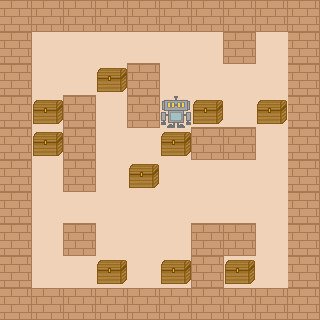
\includegraphics[scale=0.6]{simple_map.png} \\
	Obrázok 1: jednoduchá mapa
\end{leftcolumn}

\begin{rightcolumn}
	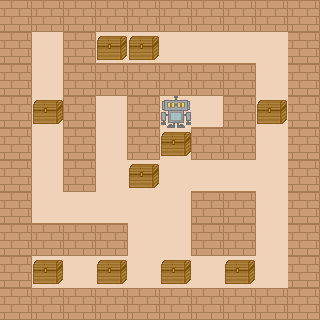
\includegraphics[scale=0.6]{complicated_map.png} \\
	Obrázok 2: komplikovaná mapa
\end{rightcolumn}
\end{paracol}
\end{center}

Budeme uvažovať zmenu nasledujúcich parametrov:

\begin{tabular}{ll}
\hline
\textsc{Population Size} & určuje veľkosť populácie po celú dobu výpočtu \\ 
\textsc{Generations} & počet generácii \\
\textsc{Crossover}  & pravdepodobnosť kríženia  \\
\textsc{Mutation}  &  pravdepodobnosť mutácie génov  \\
\textsc{MinBound \& MaxBound}  &  minimálna a maximálna dĺžka trasy robota \\ \hline
\end{tabular}

Pohyb robota na mape je reprezentovaný červenou farbou tak, že opakovaný priechod určitým miestom sposobí silnejšie červené zafarbenie. Tým ukážeme, kadiaľ robot prešiel, a zároveň kde robil zbytočné kroky navyše.

\section{Výsledky}

Pre jednoduchosť sme počas analýzy nemenili parameter veľkosti populácie. Ten je vo všetkých behoch rovný 100. Ďalej nemení horné a dolné ohraničenie dĺžky cesty. Všetky cesty sú dlhé $20-60$ symbolov. Definujeme dve rôzne fitness funkcie a pre každú identifikujeme, pri akých pravdepodobnostiach kríženia a mutácie funguje najlepšie. 


\subsection{Výsledky na základe fitness funkcií}
\textbf{1.stratégia}\\
Ako prvú sme otestovali asi najintuitívnejší prístup. Robot dostal nasledujúce ohodnotenia za svoje kroky:
\begin{itemize}
\item nenarazíš na stenu ale nenájdeš poklad : 1 bod
\item narazíš na stenu : -5 bodov
\item nájdeš poklad : 15 bodov
\end{itemize}
Táto stratégia reprezentuje to, že robota odmeníme ak nájde poklad, a potrestáme, ak narazí do steny. Aby sa po iteráciach neusadil na jednej lokálne dobrej možnosti, odmeníme ho aj za to že chodí. Pri veľmi malom pomere odmeny za poklad a chodenie však táto stratégia spôsobí neustále chodenie dookola, čo nebolo cieľom.

\noindent Túto stratégiu sme použili na oba typy máp, kde vstupné parametre boli:\\

\textsc{Population Size} = 100 \textsc{Generations} = 4000 \textsc{Crossover} = 0.7 \textsc{Mutation} = 0.3 resp. 0.4 

 
\begin{center}
  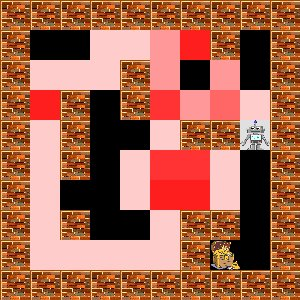
\includegraphics[scale=0.5]{strategy1_simple.jpg} 
  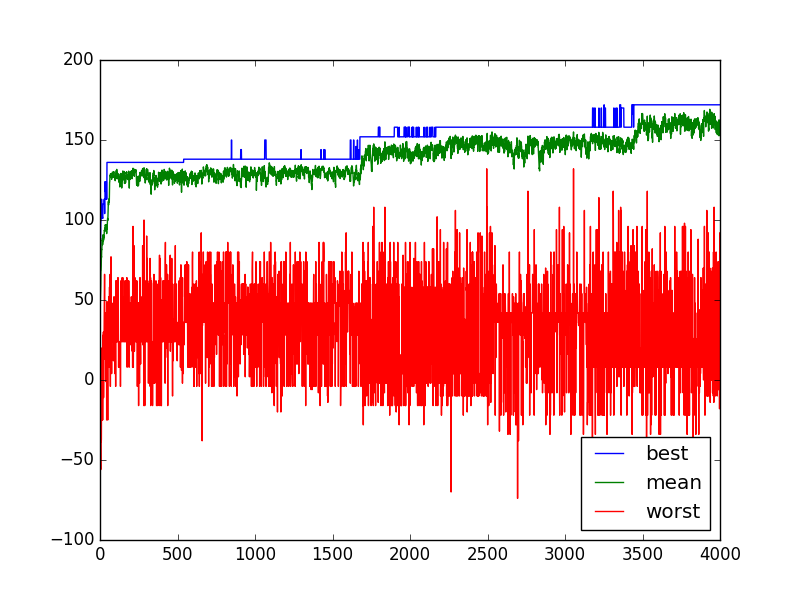
\includegraphics[scale=0.38]{strategy1_simple_graph.png} \\
   \textbf{Jednoduché bludisko}: najlepšia cesta, proces učenia
     \end{center}
     
\begin{center}
  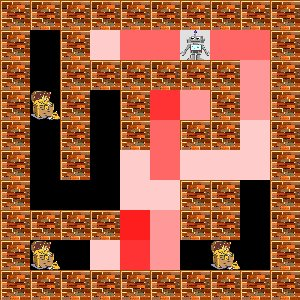
\includegraphics[scale=0.5]{strategy1_complicated.jpg} 
  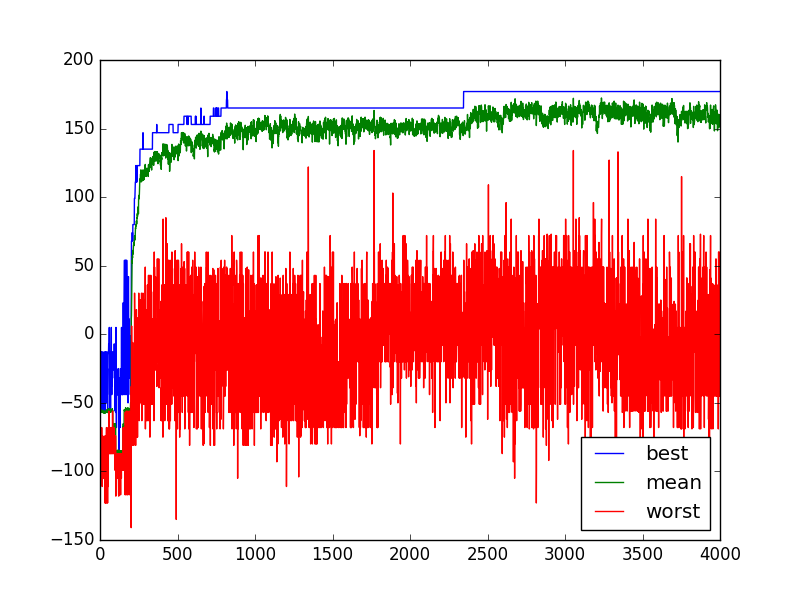
\includegraphics[scale=0.38]{strategy1_complicated_graph.png} \\
   \textbf{Kompikované bludisko}: najlepšia cesta, proces učenia
     \end{center}
     
\textit{Vyhodnotenie:} Výsledky ukazujú, že na jednoduchej mape sa bol robot schopný pomerne dobre naučiť sa nájsť poklad. Naopak, komplikované bludisko mu robilo väčšie problémy. Na kompikovanom bludisku sme skúsili aj upravené parametre, väčšiu náhodnosť mutácii, aby boli objavené iné možnosti, ako aj zvyšovanie boundu na dĺžku cesty, avšak výsledok dosiahnutý s danými parametrami považujeme za najlepší. Daná stratégia teda pre komplikované bludisko nie je vhodná. \\

\textbf{2.stratégia}\\
Ako ďaľšiu sme otestovali asi nasledovný prístup:
\begin{itemize}
\item nenarazíš na stenu ale nenájdeš poklad : 0 bodov
\item narazíš na stenu : 0 bodov
\item nájdeš poklad : 1 bod
\end{itemize}
Táto stratégia reprezentuje to, že robota odmeníme len ak nájde poklad, a teda sa predpokladá, že by sa ich mal pokúsiť nájsť čo najviac. Táto stratégia sa považuje za jednoduchšiu, a preto sme ju spustili len na 1000 iteráciach.

\noindent Túto stratégiu sme použili na oba typy máp, kde vstupné parametre boli:\\

\textsc{Population Size} = 100 \textsc{Generations} = 1000  \textsc{Crossover} = 0.6  \textsc{Mutation} = 0.4

\begin{center}
  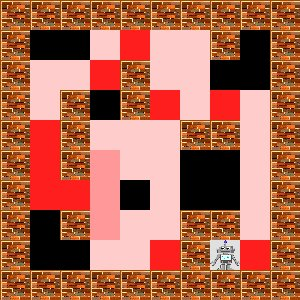
\includegraphics[scale=0.5]{strategy2_simple.jpg} 
  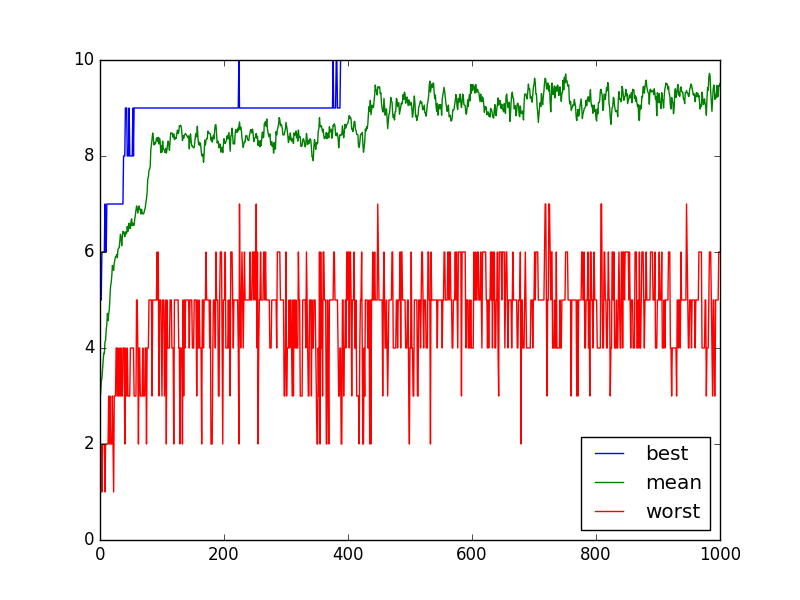
\includegraphics[scale=0.38]{strategy2_simple_graph.png} \\
   \textbf{Jednoduché bludisko}: najlepšia cesta, proces učenia
     \end{center}
     
\begin{center}
  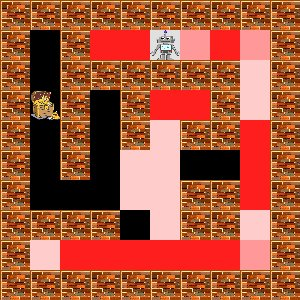
\includegraphics[scale=0.5]{strategy2_complicated.jpg} 
  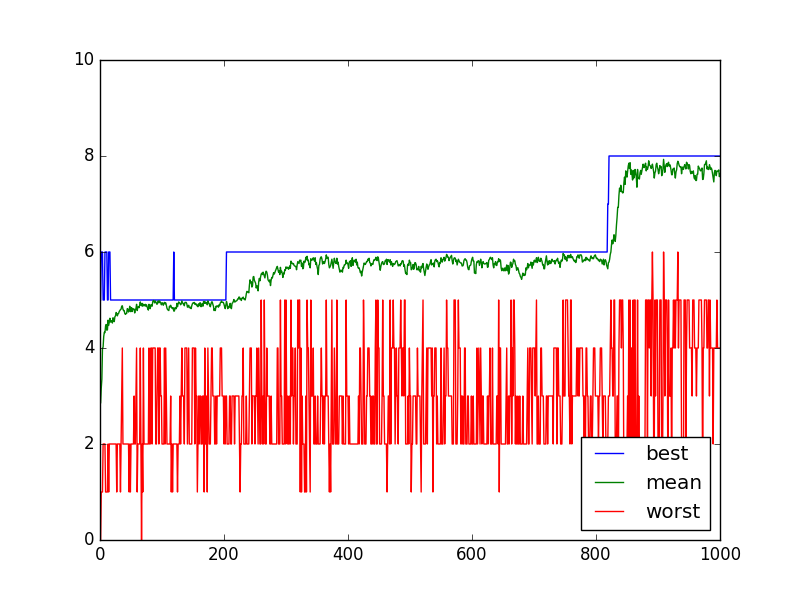
\includegraphics[scale=0.38]{strategy2_complicated_graph.png} \\
   \textbf{Kompikované bludisko}: najlepšia cesta, proces učenia
     \end{center}
     
\textit{Vyhodnotenie:} Maximálny možný počet obdov dosiahnuteľný pri tejto stratégii bol 10. Výsledky ukazujú, že robot má pre danú stratégiu dobré výsledky na oboch typoch máp. Túto stratéiu teda považujeme za veľmi efektívnu v porovnaní s jej jednoduchosťou. Ukázané výsledky predstavujú najlepší beh z 5, kde priemerné sú väčšinou o 1-2 poklady horšie.

\newpage
\subsection{Parametrizácia vstupných parametrov}

Pre obe mapy sme nagenerovali rovnaku iniciálnu populáciu a sledovali sme, ako vstupné parametre ovplyvnia dané výsledky. Minimálna a maximálna dĺžka trasy ostala po celú dobu rovnaká, tak isto ako aj veľkosť populácie. Každý beh sme spustili 4 krát a výsledky spriemerovali. 

\subsubsection{Jednoduché bludisko}

\textbf{1.stratégia}

Najprv sme testovali závislosti na kombinácii pravdepodobností kríženia a mutácie.\\
\begin{center}
\begin{tabular}{|llll|lll|}
\hline
\textsc{Population} & \textsc{Generations} & \textsc{Crossover} & \textsc{Mutation}  & best & mean & worst \\ \hline
100 & 1000 & 0.8 & 0.2 & 164.5 & 158.82 & 33.5\\ 
100 & 1000 & 0.8 & 0.4 & 170.25 & 157.24 & 66.75\\
100 & 1000 & 0.6 & 0.2 & 167.25 & 155.98 & 65.25\\
100 & 1000 & 0.6 & 0.4 & 206.75 & 178.25 & 29.0\\ \hline
\end{tabular}
\end{center}

Potom sme vybrali najúspešnejšiu stratégiu a skúmali sme ako je ovplyvnená počtom iterácií.

\begin{center}
\begin{tabular}{|llll|lll|}
\hline
\textsc{Population} & \textsc{Generations} & \textsc{Crossover} & \textsc{Mutation}  & best & mean & worst \\
100 & 100 & 0.6 & 0.4 & 154.25 &   131.84 &   37.5 \\
100 & 500 & 0.6 & 0.4 & 175.25  & 149.83 & 22.75\\
100 & 1000 & 0.6 & 0.4 & 206.75 & 178.25 & 29.0\\ 
100 & 2000 & 0.6 & 0.4 & 200.75 & 171.31 & 33.5\\
100 & 4000 & 0.6 & 0.4 & 194.25 & 167.56 & 53.5\\ \hline

\end{tabular}
\end{center}

\textbf{2. stratégia}

Najprv sme testovali závislosti na kombinácii pravdepodobností kríženia a mutácie.\\
\begin{center}
\begin{tabular}{|llll|lll|}
\hline
\textsc{Population} & \textsc{Generations} & \textsc{Crossover} & \textsc{Mutation}  & best & mean & worst \\ \hline
100 & 1000 & 0.8 & 0.2 & 7.5 & 7.36 & 4.5\\ 
100 & 1000 & 0.8 & 0.4 & 8.25 & 8.12 & 5.75\\
100 & 1000 & 0.6 & 0.2 & 9.0 & 8.56 & 4.25\\
100 & 1000 & 0.6 & 0.4 & 8.75 & 8.185 & 4.5\\ \hline
\end{tabular}
\end{center}

Potom sme vybrali najúspešnejšiu stratégiu a skúmali sme ako je ovplyvnená počtom iterácií.

\begin{center}
\begin{tabular}{|llll|lll|}
\hline
\textsc{Population} & \textsc{Generations} & \textsc{Crossover} & \textsc{Mutation}  & best & mean & worst \\
100 & 100 & 0.6 & 0.2 & 8.25 &  7.53 &  4.75 \\
100 & 500 & 0.6 & 0.2 & 8.25 & 7.92 & 4.75\\
100 & 1000 & 0.6 & 0.2 & 9.0 & 8.56 & 4.25\\ 
100 & 2000 & 0.6 & 0.2 & 9.25 & 8.97 & 4.0\\
100 & 4000 & 0.6 & 0.2 & 8.25 & 7.98 & 4.25\\ \hline
\end{tabular}
\end{center}

\textit{Vyhodnotenie:} blablablabla


\newpage 

\subsubsection{Komplikované bludisko}

\textbf{1.stratégia}

Najprv sme testovali závislosti na kombinácii pravdepodobností kríženia a mutácie.\\
\begin{center}
\begin{tabular}{|llll|lll|}
\hline
\textsc{Population} & \textsc{Generations} & \textsc{Crossover} & \textsc{Mutation}  & best & mean & worst \\ \hline

100 & 1000 & 0.8 & 0.2 & 130.5 & 126.08 & 40.25\\ 
100 & 1000 & 0.8 & 0.4 & 158.25 & 147.49 & 61.5\\
100 & 1000 & 0.6 & 0.2 & 147.0 & 137.4 & 22.25\\
100 & 1000 & 0.6 & 0.4 & 156.75 & 135.8725 & -11.75\\ \hline
\end{tabular}
\end{center}

Potom sme vybrali najúspešnejšiu stratégiu a skúmali sme ako je ovplyvnená počtom iterácií.

\begin{center}
\begin{tabular}{|llll|lll|}
\hline
\textsc{Population} & \textsc{Generations} & \textsc{Crossover} & \textsc{Mutation}  & best & mean & worst \\
 
100 & 100 & 0.8 & 0.4 & 103.5 & 87.77 & 31.55 \\
100 & 500 & 0.8 & 0.4 & 136.5 & 124.5 & 18.5\\
100 & 1000 & 0.8 & 0.4 & 158.25 & 147.49 & 61.5\\ 
100 & 2000 & 0.8 & 0.4 & 147.75 & 139.68 & 23.0\\
100 & 4000 & 0.8 & 0.4 & 167.25 & 158.38 & 68.25\\ \hline

\end{tabular}
\end{center}

\textbf{2. stratégia}

Najprv sme testovali závislosti na kombinácii pravdepodobností kríženia a mutácie.\\
\begin{center}
\begin{tabular}{|llll|lll|}
\hline
\textsc{Population} & \textsc{Generations} & \textsc{Crossover} & \textsc{Mutation}  & best & mean & worst \\ \hline

100 & 1000 & 0.8 & 0.2 & 6.5 & 6.43 & 5.25\\ 
100 & 1000 & 0.8 & 0.4 & 7.0 & 6.87 & 5.0\\
100 & 1000 & 0.6 & 0.2 & 6.5 & 6.3625 & 3.5\\
100 & 1000 & 0.6 & 0.4 & 7.5 & 7.30 & 4.5\\ \hline
\end{tabular}
\end{center}

Potom sme vybrali najúspešnejšiu stratégiu a skúmali sme ako je ovplyvnená počtom iterácií.

\begin{center}
\begin{tabular}{|llll|lll|}
\hline
\textsc{Population} & \textsc{Generations} & \textsc{Crossover} & \textsc{Mutation}  & best & mean & worst \\
100 & 100 & 0.6 & 0.2 & 6.25 & 5.95 & 3.5 \\
100 & 500 & 0.6 & 0.2 & 7.25 & 7.02 & 4.0\\
100 & 1000 & 0.6 & 0.2 & 7.5 & 7.30 & 4.5\\ 
100 & 2000 & 0.6 & 0.2 & 7.5 & 7.29 & 5.0\\
100 & 4000 & 0.6 & 0.2 & 7.5 & 7.23 & 4.25\\ \hline
\end{tabular}
\end{center}

\textit{Vyhodnotenie:} blablablabla

\section{Záverečný pokec}

Sme krásne a skvele!

\end{document}\grid
